\section{The Proposed ProTuner Scheduler}
Our MDP is defined by actions that correspond to intermediate scheduling decisions and states that represent intermediate schedules. The cost is the execution time of the schedule. To enumerate the possible schedules and evaluate their costs we use the same techniques used in~\cite{adams2019learning}. Given an n-dimensional tensor the scheduling is split to n stages and starting from the last stage and back to the input, a new scheduling decision is made at each stage, which proposes a new tiling and a compute and storage granularity at which to insert the new stage. The new tilings can be unrolled or spread across parallel threads or single instruction multiple data (SIMD) lanes. The costs of the complete schedules (at the end of simulation) are evaluated using a cost model trained on random programs that are fully scheduled. 
\begin{figure}[!t]
    \centering
    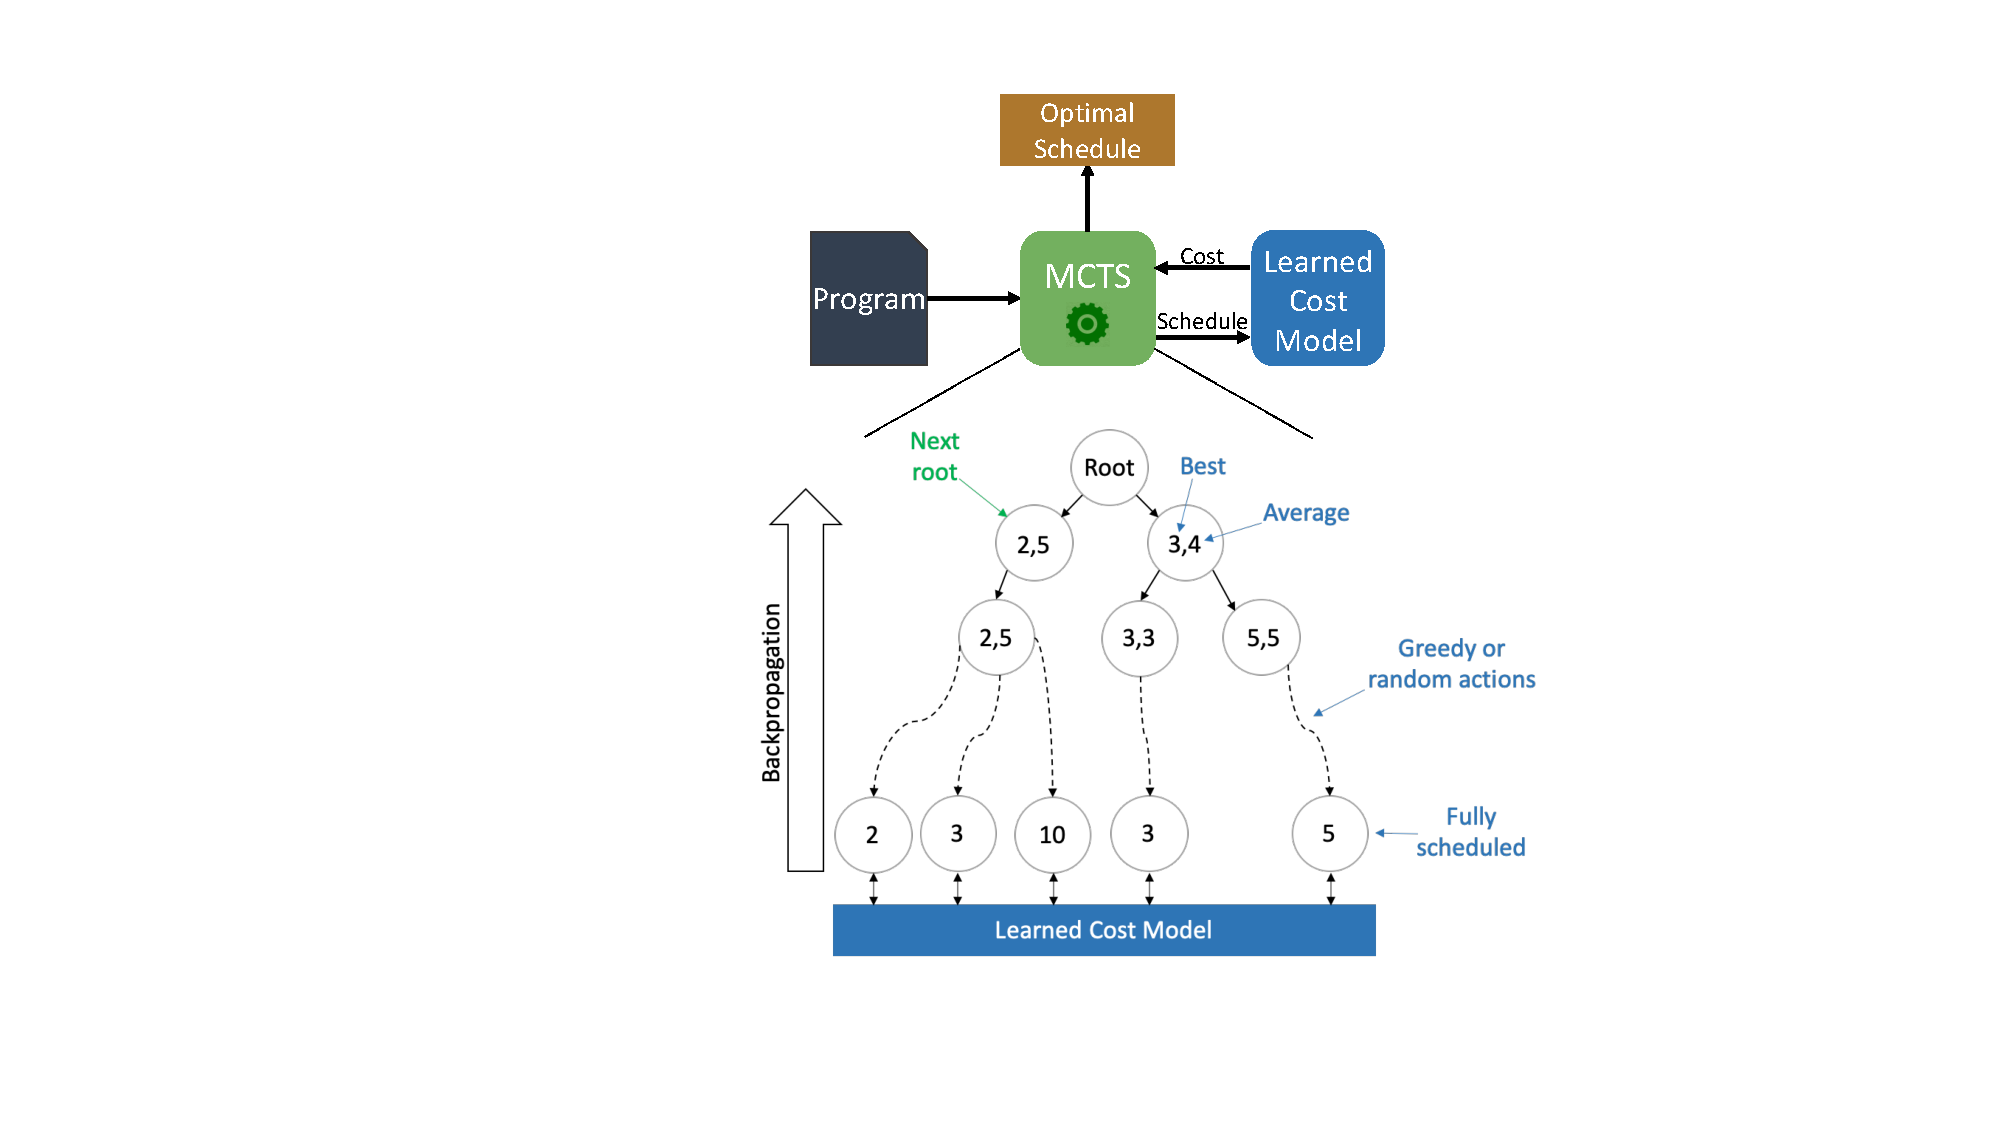
\includegraphics[width=0.5\textwidth,trim={12.7cm 2.5cm 7.5cm 1cm},clip]{figures/design.pdf}
    \caption{The block diagram of ProTuner. The program is fed to the MCTS that interacts with the learned cost model to find the optimal schedule. To make each intermediate scheduling decision the MCTS explores the benefits of the possible next actions based on the average cost but eventually picks the root that leads to the best cost. Each node stores the average costs, the best cost so far, and the complete schedule that has this best cost. The simulation can either be greedy or random. The backpropagation returns costs or 0/1 based on whether it outperforms the global best. When running an ensemble of MCTSes, the next root is picked to be the best from all the best roots.}
    \label{fig:design}
\end{figure}
\begin{figure*}[!t]
    \centering

    \begin{subfigure}[t]{0.45\textwidth}
        \centering
        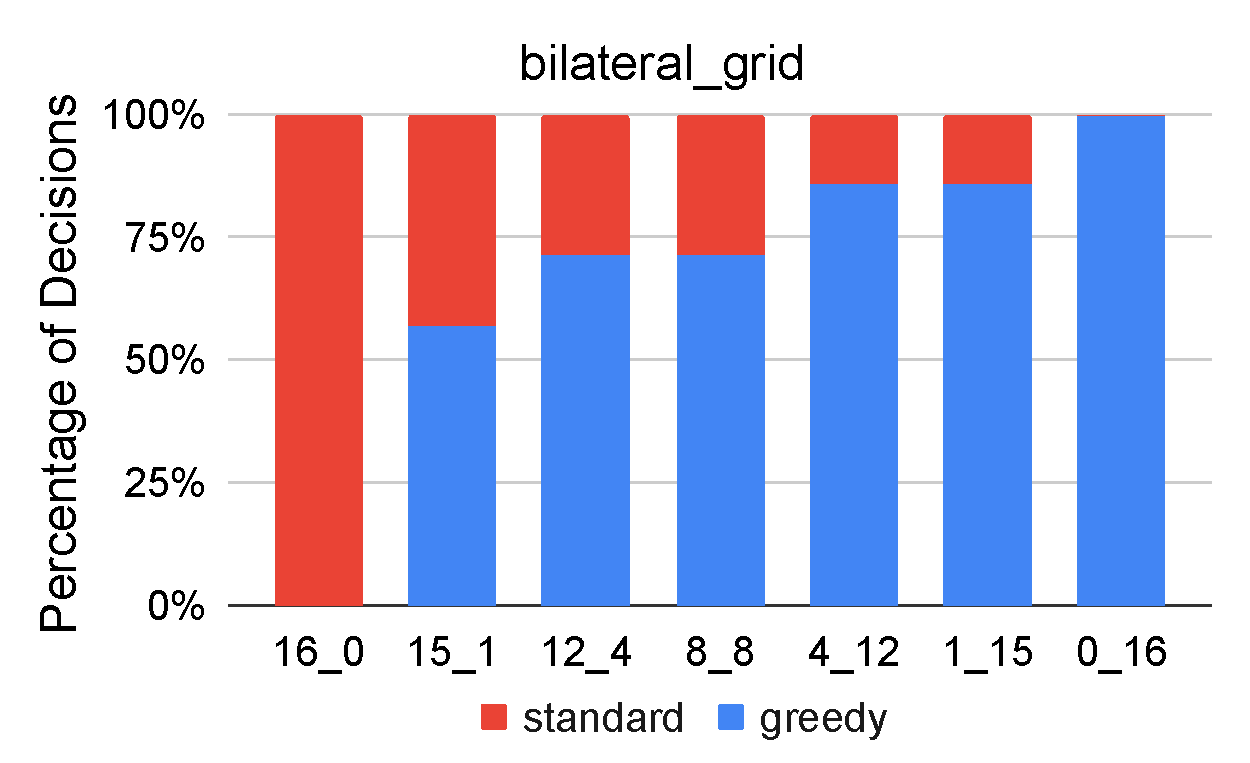
\includegraphics[width=\textwidth]{figures/bilateral_grid_random_to_greedy_ratio.pdf}
        \caption{Proportion of decisions made by standard and greedy MCTSes on the \texttt{bilateral\_grid} test.}
    \end{subfigure}
    \hspace{0.05\textwidth}
    \begin{subfigure}[t]{0.45\textwidth}
        \centering
        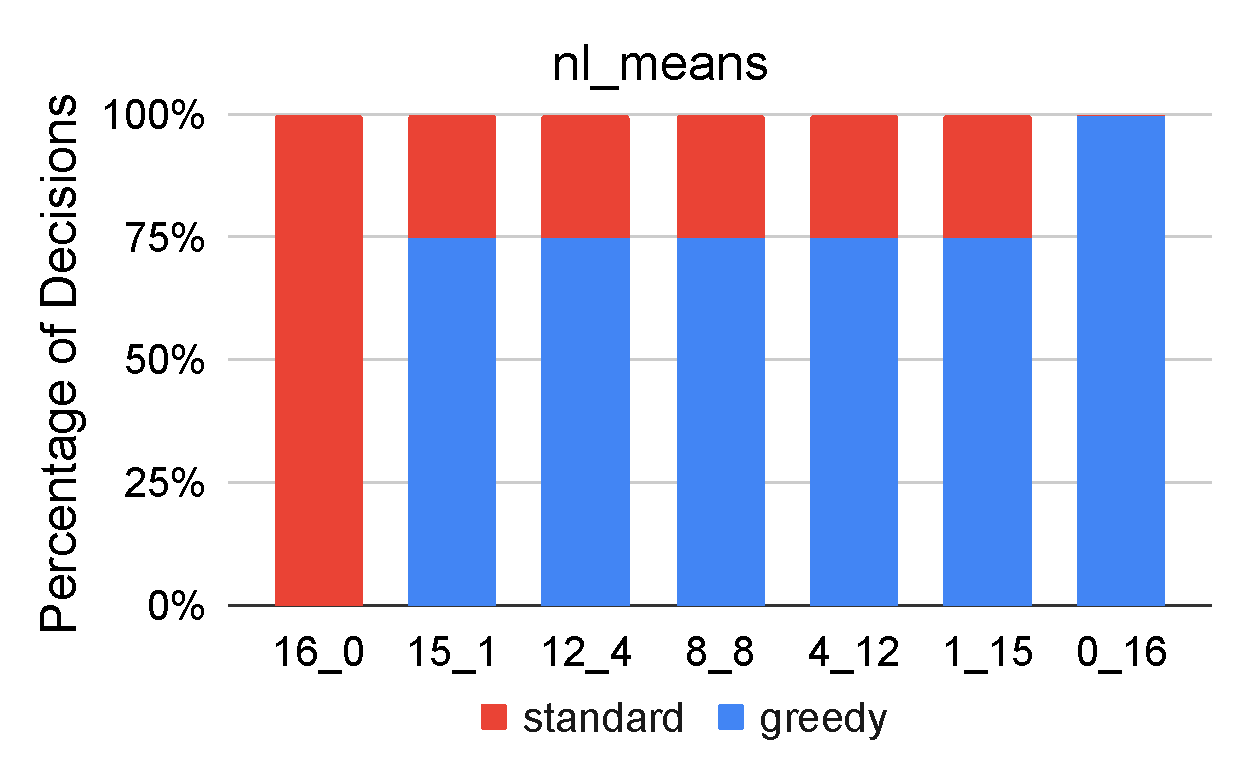
\includegraphics[width=\textwidth]{figures/nl_means_random_to_greedy_ratio.pdf}
        \caption{Proportion of decisions made by standard and greedy MCTSes on the \texttt{nl\_means} test.}
    \end{subfigure}
    
    \begin{subfigure}[t]{0.45\textwidth}
        \centering
        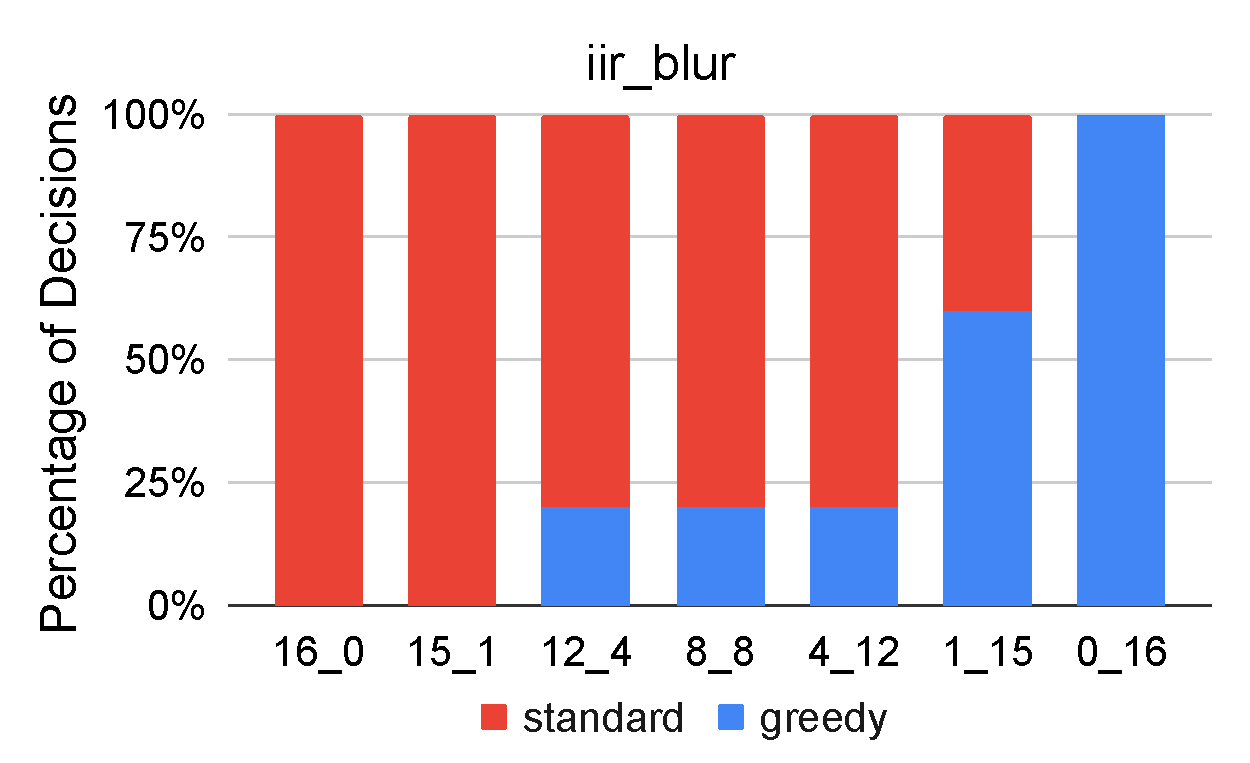
\includegraphics[width=\textwidth]{figures/iir_blur_random_to_greedy_ratio.pdf}
        \caption{Proportion of decisions made by standard and greedy MCTSes on the \texttt{iir\_blur} test.}
    \end{subfigure}
    \hspace{0.05\textwidth}
    \begin{subfigure}[t]{0.45\textwidth}
        \centering
        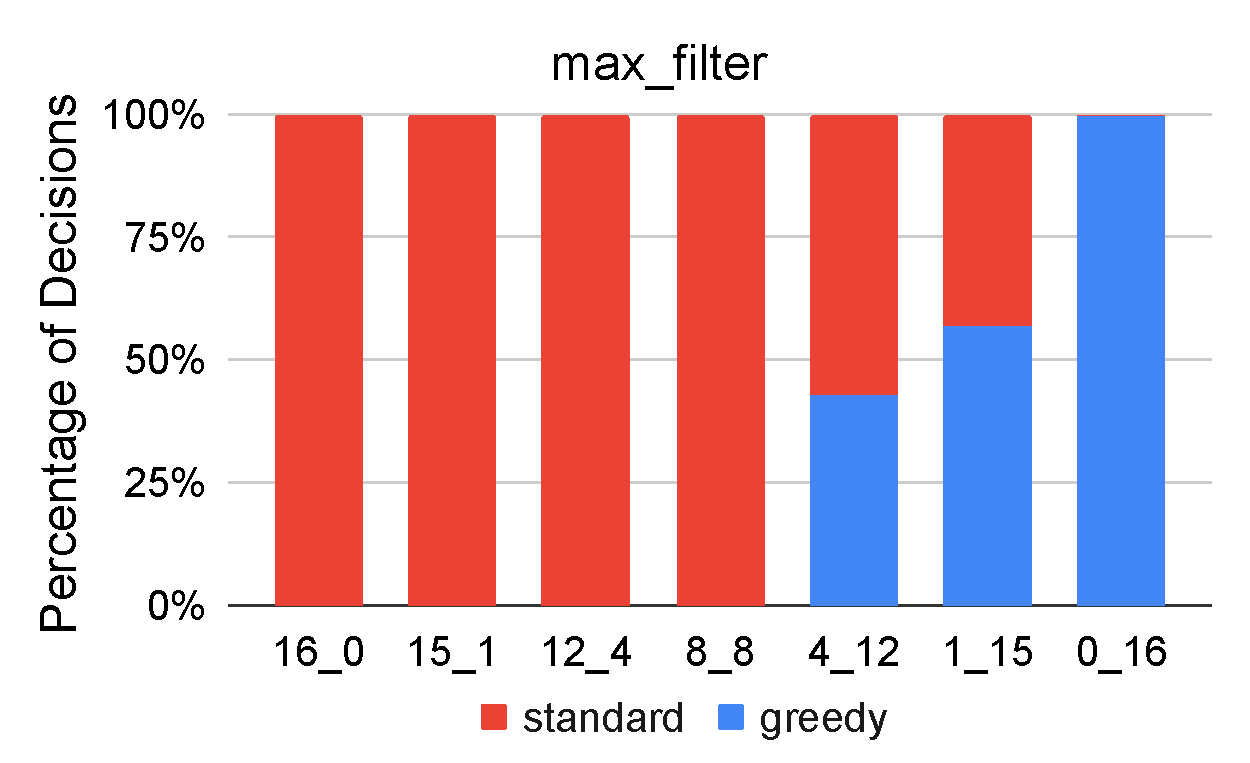
\includegraphics[width=\textwidth]{figures/max_filter_random_to_greedy_ratio.pdf}
        \caption{Proportion of decisions made by standard and greedy MCTSes on the \texttt{max\_filter} test.}
    \end{subfigure}
  
  \caption{The portion of decisions made by greedy MCTSes for a different number of standard and greedy MCTSes on a suite of four real applications. X\_Y corresponds to X standard MCTSes and Y greedy MCTSes. The overall number of trees is 16.}
  
  \label{fig:random_greedy_ratio}
\end{figure*}

Figure~\ref{fig:design} shows the block diagram of ProTuner. The MCTS starts from the last stage and explores the possible schedules back to the inputs. At every simulation from one node in the MCTS the simulation ends by computing the cost from the cost model and the cost is backpropagated to the parent nodes with the terminating fully scheduled state. These nodes update the future best cost so far, the terminating state and the value function that stores the \emph{average} cost so far. During the search the MCTS uses the average cost to determine the next child to explore. We explored the option to use the best cost in the search but that resulted in non-smooth value functions where the children that got lucky earlier and found better costs received significantly more simulations than less lucky children. This often results in a greedy behavior we are trying to avoid. 

When the computation budget is reached either after passing the number of allowed iterations or due to time out a winning action (schedule) for the current stage is determined and the new root is the state this action leads too. The winner is determined based on the \emph{best} cost so far as in \cite{bjornsson2009cadiaplayer}. We found this to outperforms taking the child with the best \emph{average} cost by 25\%. This is mainly because it can guarantee that later steps need to find schedules that are better than the best so far (rather than average best), which can be helpful when fewer iterations are available. This also allows us to combine real execution time measurements with cost model predictions at a negligible overhead.

To further improve our results we run multiple MCTSes in parallel across multiple cores that synchronize when picking a new root at every intermediate scheduling decision, which is the best child from all the best children of all the MCTSes. In addition to the performance benefits achieved from this parallelism, an ensemble of MCTSes is proven to outperform a single MCTS with the number of iterations equal to the combined number of iterations available in the ensemble~\cite{chaslot2008parallel}.

Since MCTS evaluates the program's cost when it is fully scheduled, the cost is more reliable than that of beam search, which evaluates costs of intermediate schedules that are not meaningful and the cost cannot properly evaluate since it was and could only be trained on fully scheduled programs. Unlike beam search, MCTS looks ahead and does not have the greedy nature of beam search. Furthermore, MCTS does not need to evaluate the costs of all the children during simulation or compute their state features (which we found to consume more than 92.3\% of the overhead in beam search). Instead it randomly and continuously picks a possible child and only evaluates one state when it is fully scheduled. 




\subsection{Improving Scheduling Time by Adding Greedy MCTSes}
We explored multiple techniques to improve the scheduling time of our MCTS. We found that adding some greediness to our algorithm makes it find good schedules in a shorter time. First, we explored adding greediness by picking the best next action with probability $\frac{1}{2}$ instead of randomly picking an action during the simulation phase in the MCTS. This however did not give us any benefits over simulating random actions. Instead, we tried to mimic the MCTS scheme in single-player games with 0/1 rewards. So when running from the first root, it finds the best cost, and then the children that later become roots get 1 point if they beat their parent's cost, otherwise 0. This normalizes the reward, simplifies the hyperparameter tuning of the cost, and forces the new roots to beat the costs of their ancestors. However, this resulted in 9\% worse performance.

What we found to work very well was combining standard MCTSes with an MCTS that simulates greedily. In the later, after the node to be expanded based on the UCB formula is determined, it is expanded with a \texttt{random} child but the simulation is done purely greedily using the cost model. To determine how many trees should simulate randomly or greedily we experimented with different numbers of random or greedy MCTSs on four real applications as shown in Figures~\ref{fig:random_greedy_ratio} and~\ref{fig:random_greedy}. We found that some applications like \texttt{bilateral\_grid} and \texttt{nl\_means} benefited from adding greedy MCTSes while \texttt{iir\_blur} and \texttt{max\_filter} did not. We also observed that it is sufficient to use a single MCTS that simulates greedily as it made a good balance between greediness and uniform exploration. Figure~\ref{fig:random_greedy_ratio} shows the number of decisions made by greedy MCTSes as a function of different numbers of random and greedy MCTSes. We observe that adding more greedy MCTSes did not change the number of decisions made by greedy MCTSes for \texttt{nl\_means}, which benefits from greediness. For \texttt{bilateral\_grid} there was a small increase in the number of decisions by greedy MCTSes as we increased the number of greedy MCTSes but this did not impact the performance as we found that greedy MCTSes often found similar best states. For \texttt{iir\_blur} and \texttt{max\_filter} that benefit mostly from standard MCTSes, adding more greedy MCTSes made a small increase in the number of decisions made by greedy MCTSes but on the other hand the performance got worse.


\begin{figure}[!t]
    \centering
    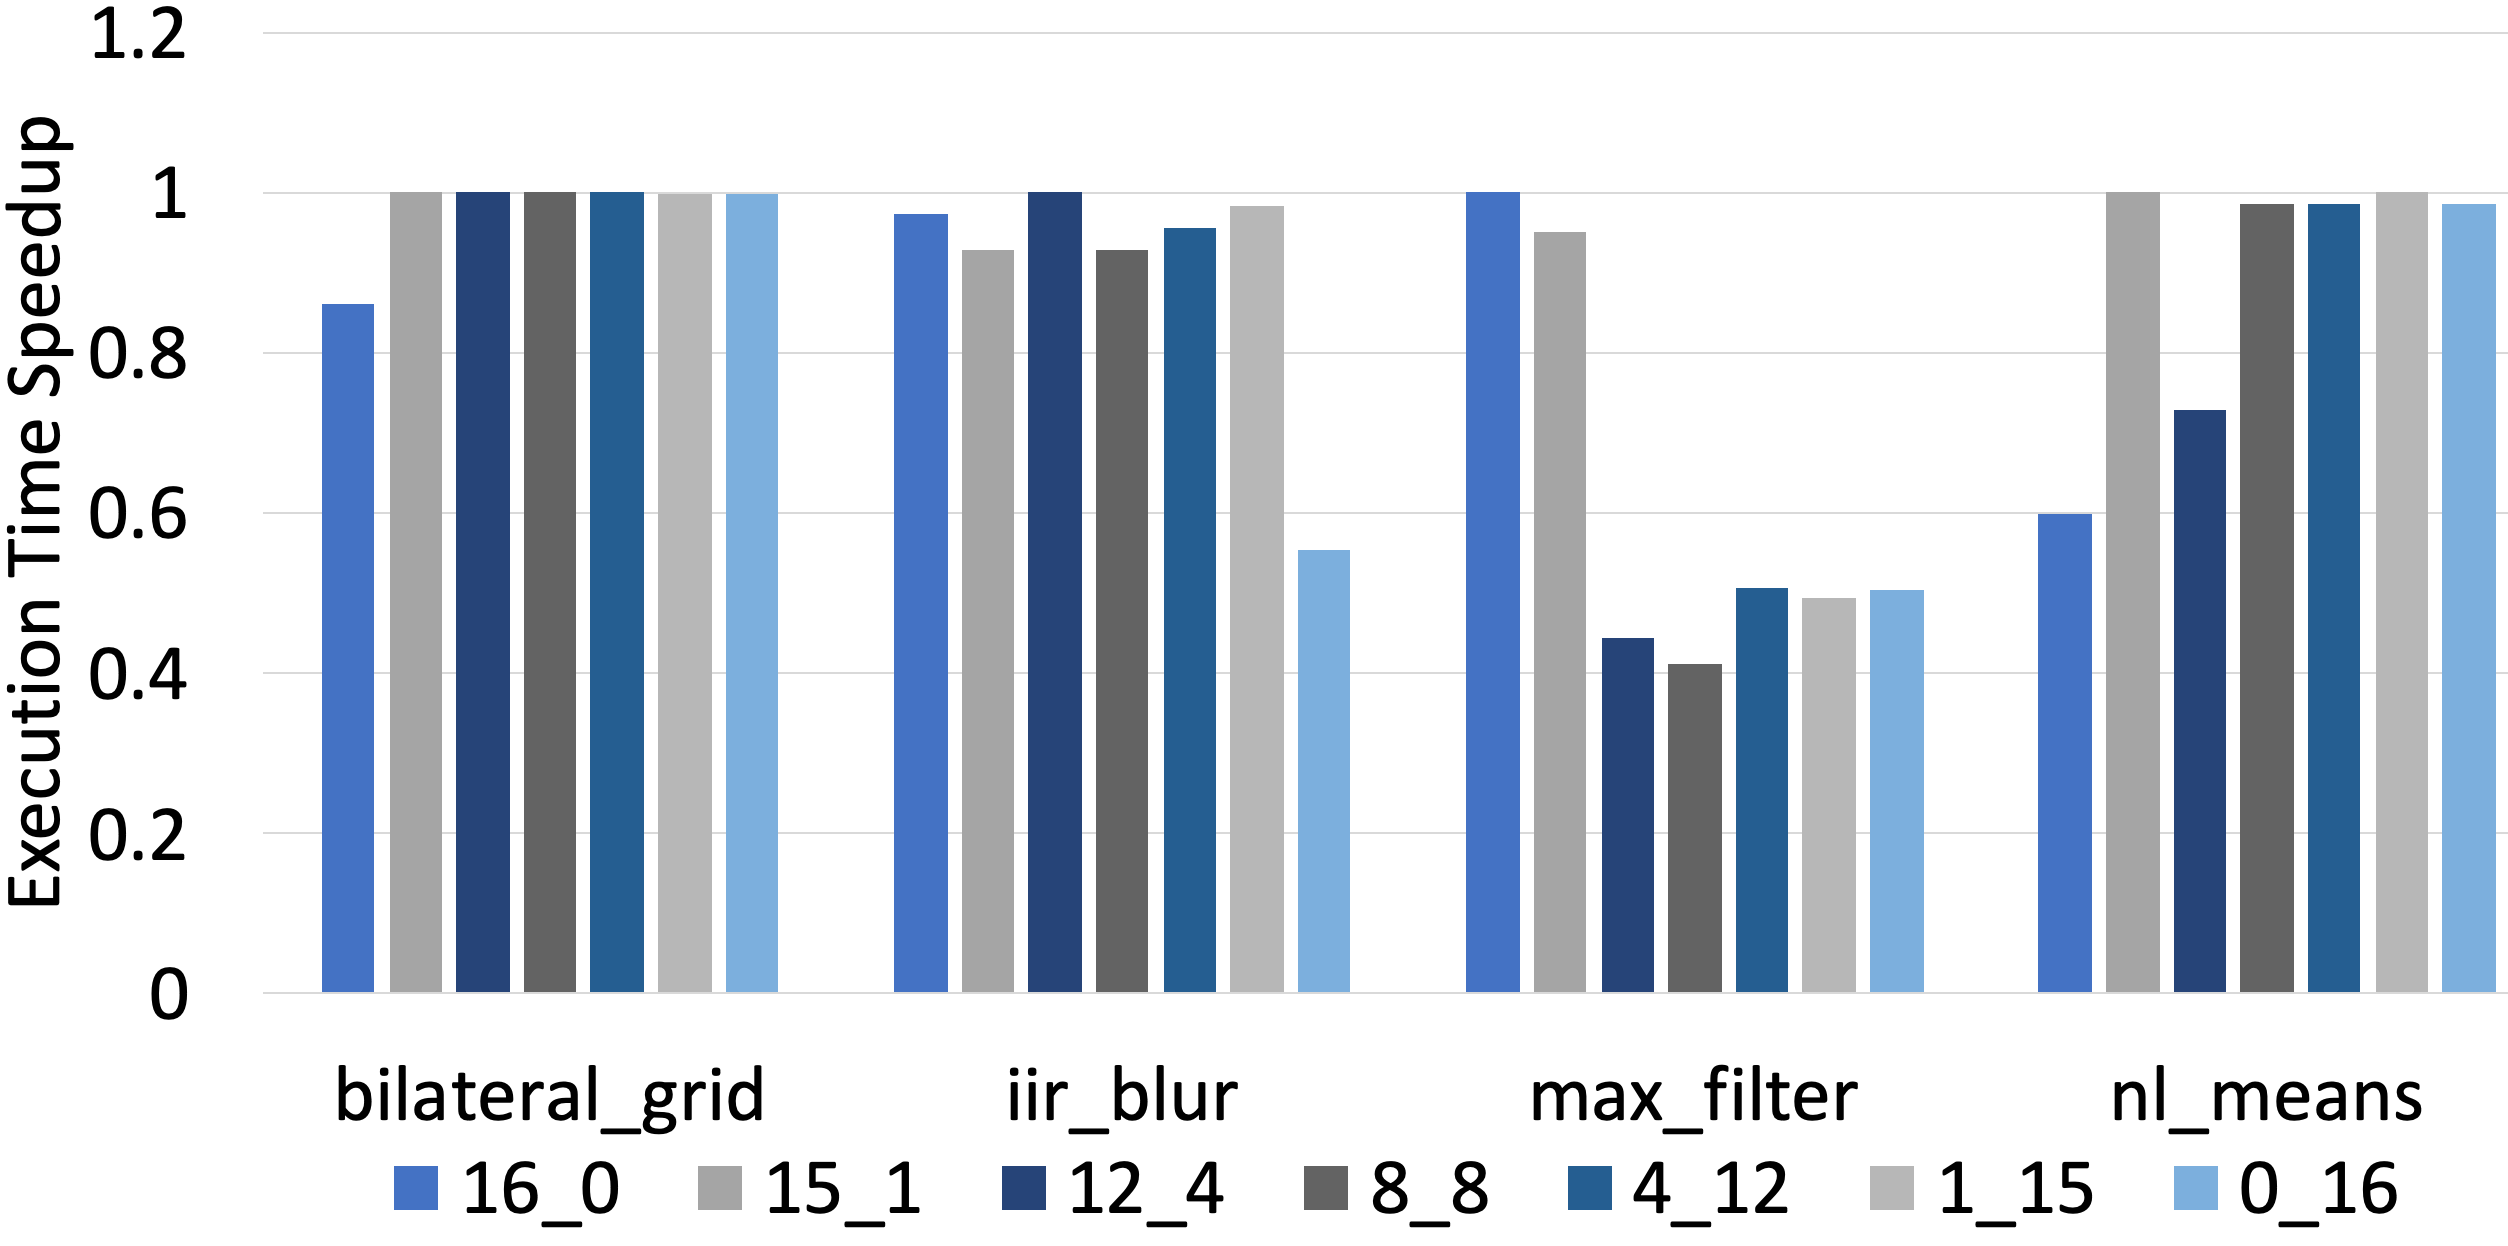
\includegraphics[width=0.48\textwidth]{figures/random_greedy4.png}
    \caption{The execution time speed up to the best execution time on a suite of four real applications (higher is better). X\_Y corresponds to X standard MCTSes and Y greedy MCTSes. The overall number of trees is 16. The 15\_1 setting did best overall.}
    \label{fig:random_greedy}
\end{figure}
\begin{figure}[!t]
    \centering
\begin{minted}{c}
all_mcts=[]
all_mcts.append(init_greedy_mcts())
all_mcts.extend(init_standard_mcts(num_mcts=15))
current_root = state0 //empty schedule
best_fully_scheduled_states={}
next_best_roots={}
while(!fully_scheduled){
  parallel_for(i=0...15){
    best_fully_scheduled_states[i], 
    next_best_roots[i] =  
        all_mcts[i].run(root=current_roots[i])
  }
  best_index = get_best_state_index_from_costs(
                    best_fully_scheduled_states)
  /* Uncomment the next lines to evaluate
  the real execution time instead of
  estimated cost:
  best_index = 
      get_best_state_index_real_measure(
        best_fully_scheduled_states) */
  parallel_for(i=0...15){
    current_roots[i] = 
        next_best_roots[best_index]
  }
  optimal_schedule = 
      best_fully_scheduled_states[best_index]
  fully_scheduled = 
      next_best_roots[best_index].is_leaf
}
\end{minted}
    \caption{Pseudocode of the MCTS scheduling algorithm that combines 15 standard MCTSes and one greedy MCTS. The best next root can be determined based on the best cost of the best fully scheduled states or based on the best execution time measurement of the best fully scheduled states as shown in the commented line.}
    \label{fig:mcts_algo}
\end{figure}
% \begin{figure}[!t]
%     \centering
%     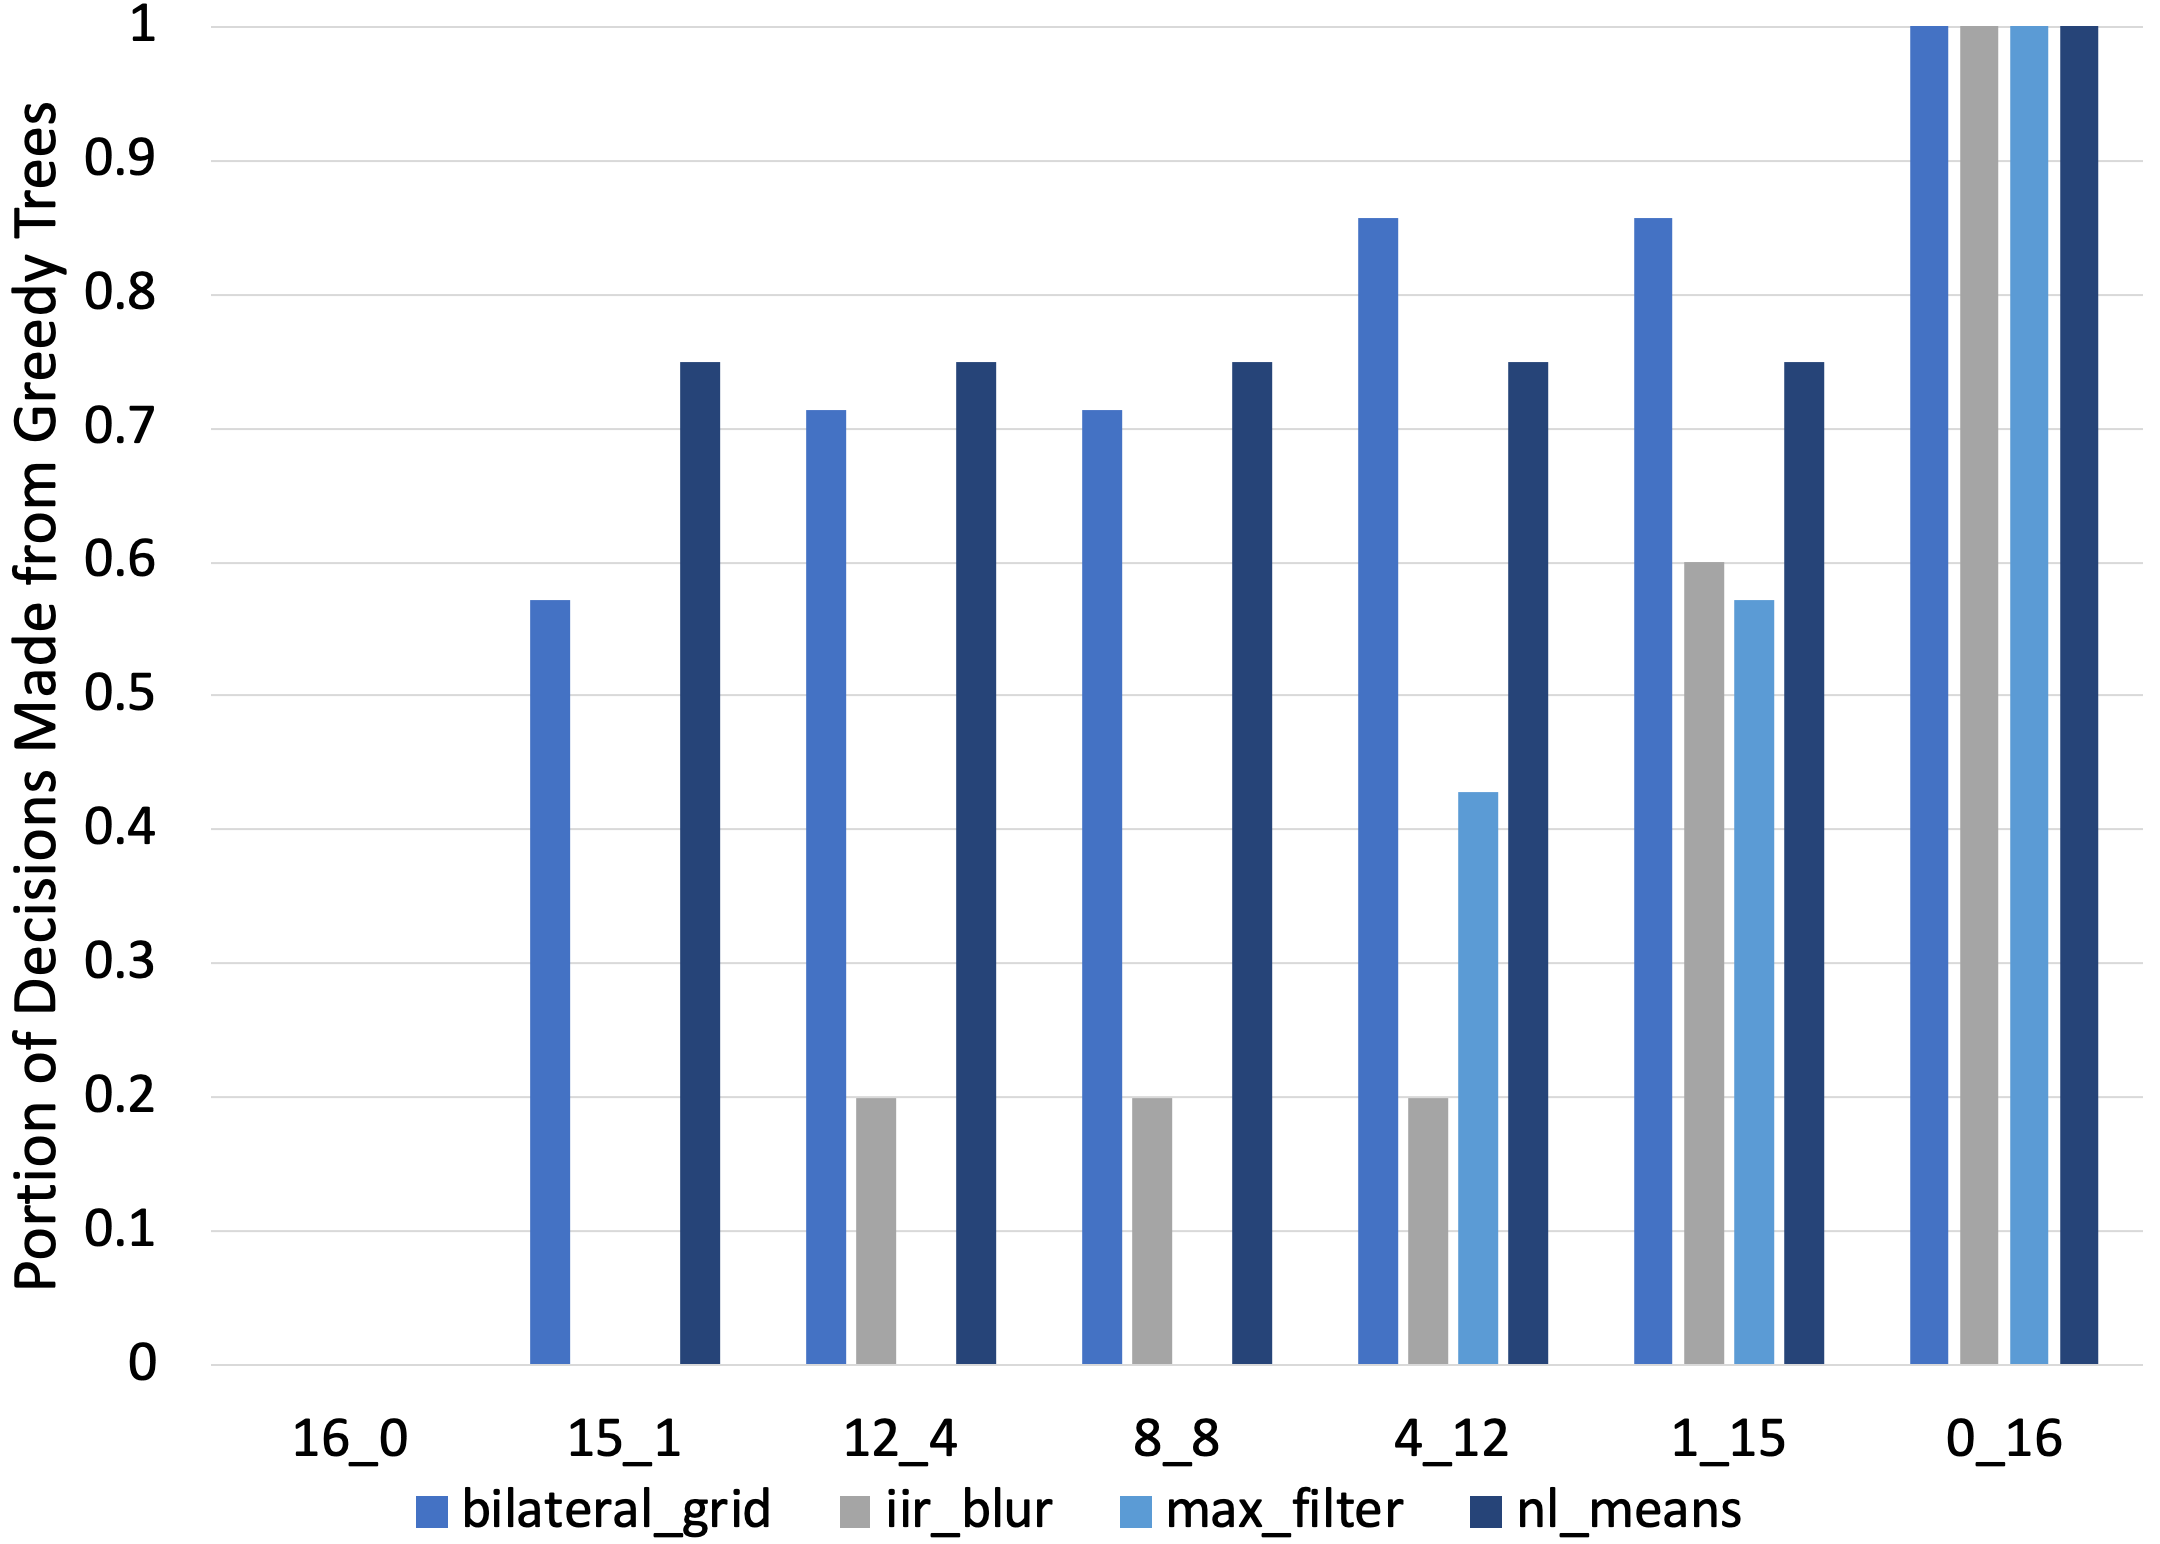
\includegraphics[width=0.48\textwidth]{figures/random_to_greedy_ratio.png}
%     \caption{The portion of decisions made by greedy MCTSes for different number of random and greedy MCTSes on a suite of four real applications. X\_Y corresponds to X standard MCTSes and Y greedy MCTSes. The overall number of trees is 16.}
%     \label{fig:random_greedy_ratio}
% \end{figure}

\begin{table*}[!t]
\centering
\begin{tabular}{|c|c|c|c|}
\hline
\textbf{Name} & \textbf{Seconds for Iteration} & \textbf{Expansion Formula} & \textbf{Measurement} \\ \hline
\texttt{mcts\_30s} & 30 & $\frac{1}{\frac{\sum_i ExecTime_i}{n_j}}(1 + \sqrt{\frac{ln(n)}{n_j}})$ & cost model \\ \hline
\texttt{mcts\_10s} & 10 & $\frac{1}{\frac{\sum_i ExecTime_i}{n_j}}(1 + \sqrt{\frac{ln(n)}{n_j}})$ & cost model \\ \hline
\texttt{mcts\_1s} & 1 & $\frac{1}{\frac{\sum_i ExecTime_i}{n_j}}(1 + \sqrt{\frac{ln(n)}{n_j}})$ & cost model \\ \hline
\texttt{mcts\_Cp10\_30s} & 30 & $\frac{1}{\frac{\sum_i ExecTime_i}{n_j}}(1 + 10\sqrt{\frac{ln(n)}{n_j}})$ & cost model \\ \hline
\texttt{mcts\_sqrt2\_30s} & 30 & $\frac{\sum_i\frac{1}{ExecTime_i}}{n_j} + \sqrt{2}\sqrt{\frac{2ln(n)}{n_j}}$ & cost model \\ \hline
\texttt{mcts\_cost+real\_30s} & 30 & $\frac{1}{\frac{\sum_i ExecTime_i}{n_j}}(1 + \sqrt{\frac{ln(n)}{n_j}})$ & \begin{tabular}[c]{@{}c@{}}cost model \\ + real\end{tabular} \\ \hline
\texttt{mcts\_cost+real\_1s} & 1 & $\frac{1}{\frac{\sum_i ExecTime_i}{n_j}}(1 + \sqrt{\frac{ln(n)}{n_j}})$ & \begin{tabular}[c]{@{}c@{}}cost model \\ + real\end{tabular} \\ \hline

\end{tabular}
\caption{The MCTS configurations explored. We explored different timeouts (time too determine a new root) in seconds per MCTS iteration, expansion formulas where we modify the UCB, and execution time measurement schemes. \texttt{mcts\_sqrt2\_30s} is the algorithm that gives the most weight to exploration and is the closest to the original UCB formula. \texttt{mcts\_Cp10\_30s} gives the second highest weight to exploration. \texttt{mcts\_cost+real\_30s} combines \texttt{mcts\_30s} from the first row and real execution time measurement. \texttt{mcts\_10s} and \texttt{mcts\_1s} reduce the seconds for iteration to ten seconds and one second, respectively. \texttt{mcts\_cost+real\_1s} combines \texttt{mcts\_1s} from the first row and real execution time measurement. \texttt{mcts\_sqrt2\_30s}, uses the original UCB formula, and encourages much more exploration than the other MCTS algorithms. We used $C_p = \frac{1}{\sqrt{2}}$ as suggested in~\cite{kocsis2006improved}, which showed that it works well with rewards in range $[0,1]$ as it satisfies the Hoeffding inequality. Multiplying the exploitation term with the exploration term encourages early exploitation.}
\label{tab:dse}
\end{table*}

\subsection{Combining the Cost Model and Real Execution Time Measurement}
Despite their inaccuracies, cost models are often used because the real measurement takes a prolonged time. To compensate for inaccuracies in the cost model while incurring minimal additional overhead, we added real execution time measurements at every iteration where a new root is declared. Our final algorithm is shown in Figure~\ref{fig:mcts_algo}. The algorithm initializes one greedy MCTS and 15 standard ones. While the program is not fully scheduled it runs the MCTSes in parallel from the current root. The returned best roots are evaluated based on the best real execution time measurement (the commented line).

To implement real execution time measurement in our C++ code the head thread \texttt{forks} multiple children. Each compiles a benchmark application serially for each of the candidate schedules returned by the greedy and standard MCTSes. Afterward, each of the compiled benchmark applications is run serially (to make sure they do not interfere with each other's run). The schedule with the best real execution time, rather than the one with the lowest cost, is used as the new root of the MCTSes for the next iteration.

To compile the benchmark applications, we used Halide's rudimentary ``RunGen'' wrapper, described in the official documentation~\cite{halide_rungen}. RunGen wraps a solitary scheduled Halide function (which is what we compiled) into a simple benchmark application that returns the execution time of the scheduled program. 

The RunGen wrapper fails to compile an error-free program for various applications, such as \texttt{camera\_pipe} and \texttt{bgu}. For these applications, we instead compiled the scheduled functions with the custom wrappers found under the \texttt{apps} directory in the official Halide repository. 

We could not use real execution time measurements for ResNet50 as it requires many simultaneously scheduled functions that a single forked child cannot run on its own. Therefore, for ResNet50, we report the results from the MCTS run that schedules it using the cost model only.
%Halide's RunGen wrapper failed to compile ResNet50 into an error-free program, but the custom wrapper code found in \texttt{apps/resnet\_50\_blockwise} could not be used either, because it requires many simultaneously scheduled functions, preventing us from benchmarking a single schedule on its own. %Therefore, we were unable to schedule ResNet50 using MCTS with the real runtimes, although we did schedule it with MCTS using the cost model.

\begin{figure*}[!t]
    \centering
    \begin{subfigure}[t]{\textwidth}
        \centering
        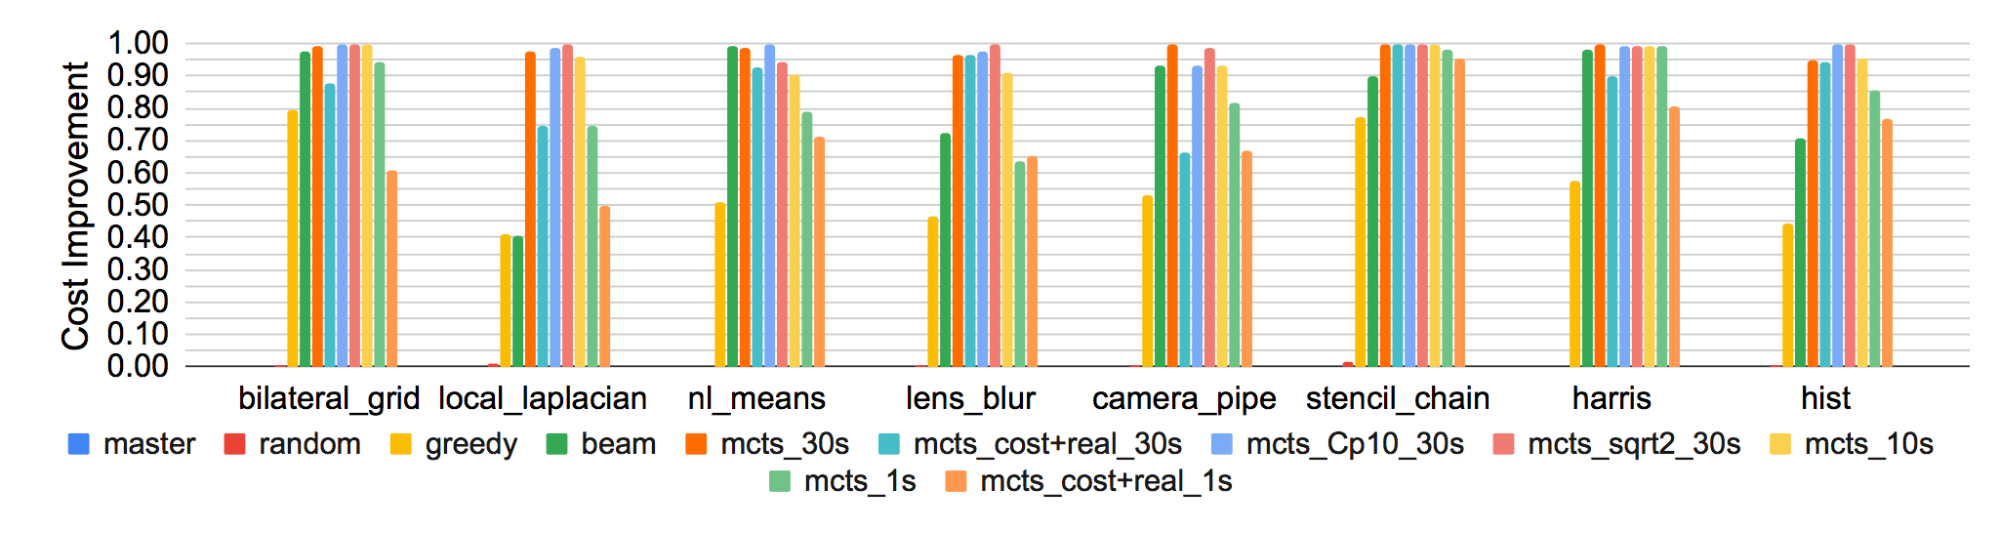
\includegraphics[trim={0cm 4.5cm 0cm 0cm},clip,width=\textwidth]{figures/cost1.png}
    \end{subfigure}
    \begin{subfigure}[t]{\textwidth}
        \centering
        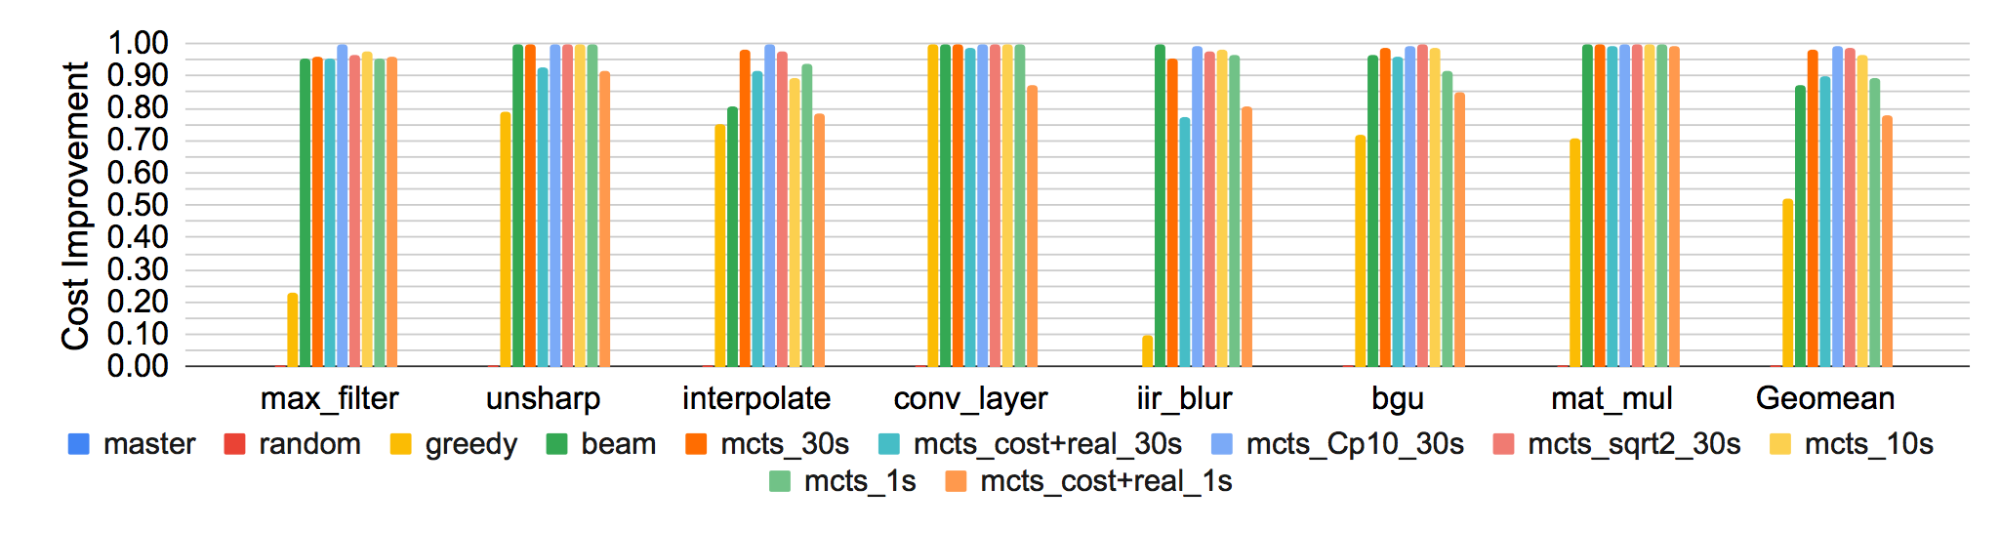
\includegraphics[width=\textwidth]{figures/cost2.png}
    \end{subfigure}
    \caption{The minimum cost found by every algorithm normalized to the best cost found by all the algorithms on a suite of 16 real benchmarks.}
    \label{fig:cost}
\end{figure*}
